%!TeX program = pdflatex
\documentclass[aspectratio=169,
10pt,
wide,
xcolor={table},
mygreen,
hyperref={colorlinks=false},
tikz]
{beamer}
\usepackage[T1]{fontenc}
\usepackage[utf8]{inputenc}

\usetheme{metropolis}
\usepackage{appendixnumberbeamer}

\usepackage{booktabs}
\usepackage{listings}
\usepackage{qrcode}

\usepackage{graphicx}
\usepackage{csquotes}
\usepackage{pgfplots}
\usepackage{pgfpages}
\usepackage{tikz}
\usepackage{svg}
\usetikzlibrary{spy, arrows, arrows.meta, shapes, shapes.multipart, fit, matrix}
\usepgfplotslibrary{dateplot}

% tikzstyles for graphs
\tikzstyle{vertex} = [circle, fill=black!25, minimum size=20pt, inner sep=0pt]
\tikzstyle{edge} = [draw, thick, -]
\tikzstyle{weight} = [font=\small]
\tikzstyle{selected vertex} = [vertex, fill=red!24]
\tikzstyle{selected edge} = [draw,line width=5pt,-,red!50]

% tikzstyles for plotting
\tikzstyle{redpoint} = [circle, fill=red, minimum size=5pt, inner sep=0pt]
\tikzstyle{bluepoint} = [circle, fill=blue, minimum size=5pt, inner sep=0pt]
\tikzstyle{dominates} = [draw, thick, -Stealth]
\tikzstyle{divides} = [draw, thick, dash pattern=on 5pt off 2pt on 1pt off 2pt]
\tikzstyle{points} = [draw, -Stealth]
\tikzstyle{ghost} = [draw=none]
\tikzstyle{barlabel} = [rectangle, behind path]

% tikzstyles for matrices
\tikzstyle{vsubmatrix} = [rectangle, fill=black!25, minimum width=10pt, minimum height=50pt]
\tikzstyle{hsupermatrix} = [matrix of math nodes, ampersand replacement=\&, column sep=1mm, left delimiter=(, right delimiter=)]
\tikzstyle{hsubmatrix} = [rectangle, fill=black!25, minimum width=50pt, minimum height=10pt]
\tikzstyle{vsupermatrix} = [matrix of math nodes, ampersand replacement=\&, row sep=1mm, left delimiter=(, right delimiter=)]

\usepackage{multicol}
\usepackage{hyperref}
\usepackage{makecell}
\usepackage{soul}

\usepackage[backend=biber, style=verbose, doi=false, isbn=false, url=false]{biblatex}
\addbibresource{pres.bib}

\definecolor{Petrol}{HTML}{066F4F}
\definecolor{Red}{HTML}{B11002}
\definecolor{Blue}{HTML}{1078B1}
\definecolor{Yellow}{HTML}{B88C09}
\definecolor{maincolor}{named}{Petrol}

\setbeamercolor{palette primary}{bg=Petrol}
\setbeamercolor{alerted text}{fg=Red}
\setbeamercolor{example text}{fg=Blue}
\setbeamercolor{block title}{fg=Petrol}
\setbeamercolor{title}{fg=Petrol}
\setbeamercolor{progress bar}{fg=Petrol}

\setbeamercolor{frame numbering}{fg=Petrol}

\setbeamertemplate{frame footer}{\color{Petrol}\insertshorttitle}
\setbeamertemplate{section in toc}[sections numbered]

\newcommand{\bet}[1]{\textbf{\color{maincolor}#1}}
\newcommand{\minor}[1]{\textcolor{black!50}{#1}}
\newcommand{\code}[1]{\texttt{#1}}
\usepackage{xspace}
\makeatletter 
\xspaceaddexceptions{\grqq \grq \csq@qclose@i \} } 
\makeatother
\usepackage{multicol}
% ===========================================================

% ===========================================================
\usepackage{xcolor}
\definecolor{fbblau}{HTML}{3078AB}
\definecolor{mediumgray}{gray}{.65}
\definecolor{blackberry}{rgb}{0.53, 0.0, 0.25}
% ===========================================================

% ===========================================================
\usepackage{marvosym} % lightning symbol
\usepackage{amsmath}
\setbeamertemplate{theorems}[numbered]
\usepackage{amssymb}
\usepackage{interval}
\intervalconfig{soft open fences}

\newcommand{\abs}[2][]{\left\lvert#2\right\rvert_{#1}}

\DeclareMathOperator*{\argmax}{arg\,max}
\DeclareMathOperator*{\argmin}{arg\,min}
% ===========================================================

% ===========================================================
\usepackage[noline, noend]{algorithm2e}
% ===========================================================

\newcommand{\hyper}[1]{\bet{\underline{\smash{#1}}}}

\renewcommand{\thead}[1]{%
	\bfseries
	\begin{tabular}{@{}c@{}}
		\vrule height 1.2\ht\strutbox width 0pt\ignorespaces
		#1
		\unskip\vrule depth 1.2\dp\strutbox width 0pt
	\end{tabular}%
}


\author{Peter Oehme}
\title{All Pairs Shortest Paths in \texorpdfstring{$\mathcal{O}(n^3 / \log(n))$}{O (n \^{} 3 / log (n))} Time}
\date{10 January 2023}

\begin{document}

\pgfdeclarelayer{background}
\pgfsetlayers{background,main}

\begin{frame}
    \maketitle
\end{frame}

\begin{frame}{Overview}
    \tableofcontents
\end{frame}

\section{Introduction to APSP}

\begin{frame}{Shortest Paths Problems\footnote{\cite[Section~24]{Cormen2001}}}
    Consider a possibly directed graph $G = (V, E)$ with weights $w \in E'$.
    We say that a path $\tilde{p} = (e_1, e_2, \dots, e_n), e_1 = (a, \cdot), e_n = (\cdot, b)$ is a \emph{shortest path} from a vertex $a$ to a vertex $b$, iff
    \[
        \tilde{p} = \argmax\limits_{p\text{ path from }a\text{ to }b} w(p),
    \]
    where $\begin{aligned}[t]w(p) = \sum\limits_{i = 1}^n w(e_i)\end{aligned}$.

    \uncover<2->{
        \begin{alertblock}{Variants}
            \begin{itemize}
                \item<2-> Single Pair Shortest Paths Problems (Fix both origin and target vertices $a$ and $b$)
                \item<3-> Single Destination Shortest Paths Problems (Fix target vertex $b$)
                \item<4-> Single Source Shortest Paths Problems (Fix origin vertex $a$)
                \item<5-> All Pairs Shortest Paths Problems
            \end{itemize}
        \end{alertblock}
    }
\end{frame}

\begin{frame}{Single Source Shortest Paths (SSSP)\footnote[1]{\cite[Section~24]{Cormen2001}}}
    \begin{columns}
        \begin{column}{0.8\textwidth}
            \begin{figure}
                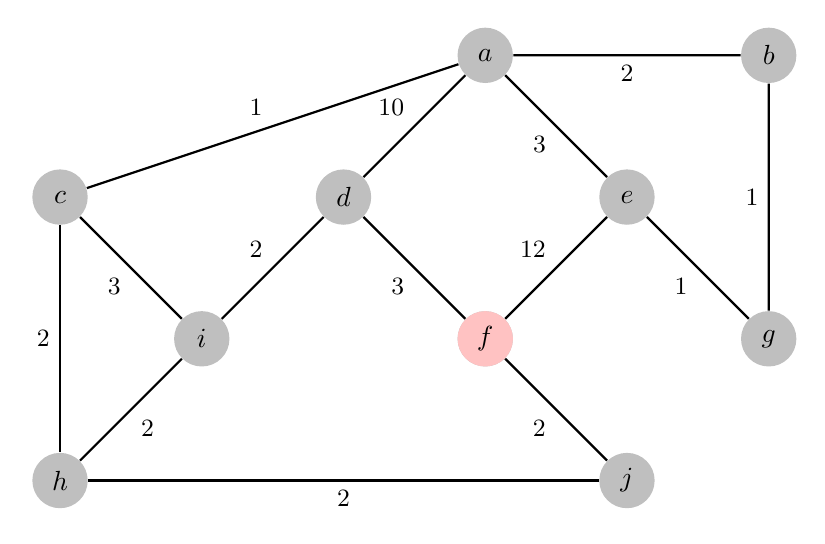
\begin{tikzpicture}[scale=0.6, auto, swap]
                    \foreach \pos / \name in {%
                        {(8, 9)/a}, {(14, 9)/b},%
                        {(-1, 6)/c}, {(5, 6)/d}, {(11, 6)/e},%
                        {(8, 3)/f}, {(14, 3)/g}, {(2, 3)/i},%
                        {(-1, 0)/h}, {(11, 0)/j}%
                    }%
                        \node[vertex] (\name) at \pos {$\name$};
        
                    \foreach \source / \dest / \weight in {%
                        a/b/2, a/c/1, a/d/10, a/e/3,%
                        b/g/1,%
                        c/h/2, c/i/3,%
                        d/f/3, d/i/2,%
                        e/f/12, e/g/1,%
                        f/j/2,%
                        h/i/2, h/j/2%
                    }%
                        \path[edge] (\source) -- node[weight] {$\weight$} (\dest);
        
                    \only<2->{
                    \foreach \vertex / \fr in {f/1}%
                        \path<\fr-> node[selected vertex] at (\vertex) {$\vertex$};
                    }
                \end{tikzpicture}
            \end{figure}
        \end{column}
        \begin{column}{0.2\textwidth}
            \only<3>{
            $\implies \begin{pmatrix}7 \\ 9 \\ 6 \\ 3 \\ 10 \\ 0 \\ 10 \\ 4 \\ 5 \\ 2\end{pmatrix}$
            $\begin{matrix}a \\ b \\ c \\ d \\ e \\ f \\ g \\ h \\ i \\ j\end{matrix}$
            }
        \end{column}
    \end{columns}
\end{frame}

\begin{frame}{Solving SSSP\footnote[1]{\cite[Section~24]{Cormen2001}}}
    \only<1>{
        \begin{exampleblock}{Assumption}
            We assume that the graph $G$ contains no negative weight cycles.

            Here a negative weight cycle refers to a path $p = (e_1, \dots, e_n)$ such that $e_1 = (a, \cdot), e_n = (\cdot, a)$ and $w(p) < 0$.
            If we are looking for a shortest path containing the vertex $a$, including a negative weight cycle always reduces the weight of the total path. \Lightning{}
        \end{exampleblock}
    }
    \only<2->{
        Among others, the \emph{Bellman-Ford} algorithm solves the SSSP problem:

        \begin{algorithm}[H]
            \KwData{Starting vertex $a$}
            Initialize $d(a) = 0, d(v) = \infty \,\forall v \in V \setminus \{ a \}$\;
            \ForEach{$v \in V \setminus \{ a \}$}{
                \ForEach{$e = (u, v) \in E$}{
                    \If{$d(v) > d(u) + w(e)$}{
                        $d(v) = d(u) + w(e)$
                    }
                }
            }
        \end{algorithm}

        \uncover<3->{
            \begin{exampleblock}{Note}
                It is easy to keep track of each nodes predecessor to later recover the shortest path to any given vertex.

                \uncover<4>{
                    Bellman-Ford can also check for the existence of negative weight cycles.\footnote[2]{\cite[Section~24.1]{Cormen2001}}
                }
            \end{exampleblock}
        }
    }
\end{frame}

\begin{frame}{All Pairs Shortest Paths (APSP)\footnote[1]{\cite[Section~25.1]{Cormen2001}}}
    \only<1, 2>{
        The \emph{All Pairs Shortest Paths} problem can be naively solved by applying Bellman-Ford to every vertex in $G$.
        However faster alternatives are available, such as making use of \emph{repeated squaring}.
        
        \uncover<2>{
            To illustrate:
            \begin{align*}
                L_1 &= W \\
                L_2 &= W \cdot W \\
                L_4 &= W^2 \cdot W^2 \\
                &\vdots \\
                L_{2^{\lceil \log(n - 1) \rceil}} &= W^{2^{\lceil \log(n - 1) \rceil - 1}} \cdot W^{2^{\lceil \log(n - 1) \rceil - 1}}
            \end{align*}
        }
    }
    \only<3, 4>{
        \begin{algorithm}[H]
            \KwData{Initialized weight matrix $W$}
            $L_1 = W, m = 1$\;
            \While{$m < n - 1$}{
                Consider $L_{m}$ to have entries $l_{i, j}$\;
                Consider $L_{2 m}$ to be a new $n \times n$ matrix with entries $l'_{i, j}$\;
                \For{$i = 1, \dots, n$}{
                    \For{$j = 1, \dots, n$}{
                        $l_{i, j} = \infty$\;
                        \For{$k = 1, \dots, n$}{
                            $l_{i, j} = \min \{ l'_{i, j}, l_{i, k} + l_{k, j} \}$
                        }
                    }
                }
                $m = 2m$\;
            }
        \end{algorithm}

        \uncover<4>{
            This takes a time of $\mathcal{O}\left( n^3 \log(n) \right)$.
        }
    }
    \only<5->{
        \only<5,6>{
            Omitting the squared matrix approach and directly calculating the updates on the matrix, we obtain the \emph{Floyd-Warshall} algorithm.
            This only takes $\mathcal{O}\left( n^3 \right)$.
        }

        \uncover<6->{
            \begin{algorithm}[H]
                \KwData{Initialized weight matrix $W$}
                $D_0 = W$ with entries $d_{i, j}$\;
                \For{$k = 1, \dots, n$}{
                    Consider $D_{k - 1}$ to have entries $d_{i, j}$\;
                    Consider $D_{k}$ to be a new $n \times n$ matrix with entries $d'_{i, j}$\;
                    \For{$i = 1, \dots, n$}{
                        \For{$j = 1, \dots, n$}{
                            $d'_{i, j} = \min \{ d_{i, j}, d_{i, k} + d_{k, j} \}$\;
                        }
                    }
                }
            \end{algorithm}
        }

        \only<7>{
            \begin{exampleblock}{Note}
                It is relatively easy to keep track of a vertex' predecessor when updating the weights, making it possible to retrieve the shortest path after runtime.
            \end{exampleblock}
        }
    }
\end{frame}

\section{APSP Algorithms with Subcubic Runtime}

\begin{frame}{asdf}
    qwer
\end{frame}
\section{Structure of the Proof}

\begin{frame}{Basic Ideas}
    The proof is structured as follows:
    \uncover<2->{
        \begin{enumerate}
            \item<2-> A problem in computational geometry\uncover<5->{$\implies$ \emph{Finding dominating pairs}}
            \item<3-> Computing products of matrices\uncover<6->{$\implies$ \emph{Sorting indices in sets}}
            \item<4-> Combining the two ideas\uncover<7->{$\implies$ \emph{Splitting matrices and multiplying them efficiently}}
        \end{enumerate}
    }
\end{frame}

\begin{frame}{Dominating Pairs}
    \begin{alertblock}{Dominating Pair}
        \only<1, 2>{
            Let $\mathfrak{M}_1, \mathfrak{M}_2$ be (finite) subsets of $\mathbb{R}^d$ with $d \in \mathbb{N}$.
            Then a \emph{dominating pair} is defined to be a tuple $(p, q) \in \mathfrak{M}_1 \times \mathfrak{M}_2$ such that it holds
            \[
                \forall k = 1, \dots, d: p_k \leq q_k,
            \]
            where $p_k$, and $q_k$ are the $k$-th coordinate of $p$, and $q$ respectively.
        }
        \only<3->{
            \begin{figure}
                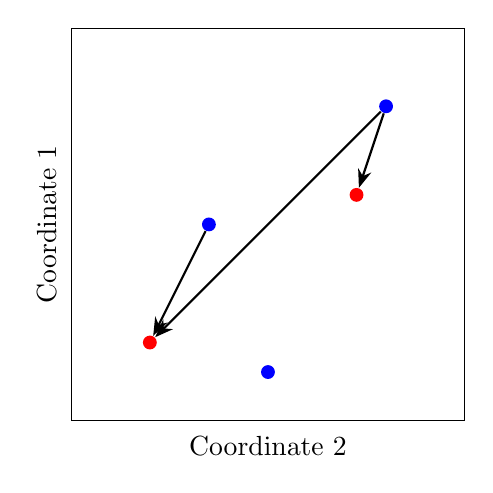
\begin{tikzpicture}[scale=0.75, auto, swap]
                    \foreach \pos / \name in {%
                        {(1, 1)/a}, {(4.5, 3.5)/b}%
                    }%
                        \node[redpoint] (\name) at \pos {};

                    \foreach \pos / \name in {%
                        {(3, 0.5)/A}, {(2, 3)/B}, {(5, 5)/C}%
                    }%
                        \node[bluepoint] (\name) at \pos {};

                    \only<4>{
                        \foreach \source / \dest in {%
                            B/a, C/a,%
                            C/b%
                        }%
                            \path[dominates] (\source) -- (\dest);
                    }

                    \node[barlabel] (labelx) at (3, -0.75) {Coordinate 2};
                    \node[barlabel, rotate=90] (labely) at (-0.75, 3) {Coordinate 1};

                    \node[ghost] (bound1) at (0, 0) {};
                    \node[ghost] (bound2) at (6, 6) {};

                    % border
                    \node[draw,fit=(bound1) (bound2)] (border) {};
                \end{tikzpicture}
            \end{figure}
        }
    \end{alertblock}
    \only<2>{
        \begin{block}{Note}
            This implies that for any dominating pair, the first point will always be the one with smaller coordinates.
            This can, to a certain degree, be seen as an ``ordering'' of $\mathfrak{M}_1$, and $\mathfrak{M}_2$.
        \end{block}
    }
\end{frame}

\begin{frame}{Lemma 2.1\autocite{Chan2007}}
    \begin{lemma}\label{lem:dom_pairs}
        Let $\mathbb{P} \subset \mathbb{R}^d$ be a set of red or blue points, partitioned into $\mathbb{P}_{red}$ and $\mathbb{P}_{blue}$ such that $n = \abs{\mathbb{P}_{red}} + \abs{\mathbb{P}_{blue}}$, and $\varepsilon \in \interval[open]{0}{1}$.
        Then we can find all $k$ dominating pairs in a time of $\mathcal{O}\left( c_\varepsilon^d n^{1 + \varepsilon} + k \right)$, where we define $c_\varepsilon := \frac{2^\varepsilon}{2^\varepsilon - 1}$.
    \end{lemma}
\end{frame}

\begin{frame}{Matrix Products}
    \begin{alertblock}{Min-Plus/Distance Product}
        We define the \emph{min-plus} or \emph{distance product} as the operator
        \[
            \otimes : \mathbb{R}^{n \times d} \times \mathbb{R}^{d \times m} \rightarrow \mathbb{R}^{n \times m},\qquad
            {\left( A \otimes B \right)}_{i, j} := \min\limits_{k \in \{ 1, \dots, d \}} a_{i, k} + b_{k, j}.
        \]
    \end{alertblock}

    \only<2->{
        \begin{columns}
            \begin{column}{.53\linewidth}
                \begin{exampleblock}{Computing Distances}
                    This product is useful, because it mimics the computation of shortest distances:
                    \begin{figure}
                        \begin{minipage}{.8\linewidth}
                            \begin{algorithm}[H]
                                \If{$d(a, c) > d(a, b) + d(b, c)$}{
                                    $d(a, c) := d(a, b) + d(b, c)$
                                }
                            \end{algorithm}
                        \end{minipage}
                    \end{figure}
                \end{exampleblock}
            \end{column}
            \begin{column}{.4\linewidth}
                \begin{figure}
                    \begin{tikzpicture}[scale=0.95, auto, swap]
                        \foreach \pos / \name in {%
                            {(0, 0)/a}, {(5, 0)/c}, {(2.5, 2)/b}%
                        }%
                            \node[vertex] (\name) at \pos {$\name$};
            
                        \foreach \source / \dest / \weight in {%
                            a/b/3, a/c/7, b/c/2%
                        }%
                            \path[edge] (\source) -- node[weight] {$\weight$} (\dest);

                        \foreach \vertex / \fr in {a/3, c/3}%
                            \path<\fr-> node[selected vertex] at (\vertex) {$\vertex$};

                        \foreach \vertex / \fr in {a/4, b/4, c/4}%
                            \path<\fr-> node[selected vertex] at (\vertex) {$\vertex$};

                        \only<3>{
                            \begin{pgfonlayer}{background}
                                \path<+->[selected edge] (a.center) -- (c.center);
                            \end{pgfonlayer}
                        }

                        \only<4>{
                            \begin{pgfonlayer}{background}
                                \foreach \source / \dest in {a/b, b/c}
                                    \path<+->[selected edge] (\source.center) -- (\dest.center);
                            \end{pgfonlayer}
                        }
                    \end{tikzpicture}
                \end{figure}
            \end{column}
        \end{columns}
    }
\end{frame}

\begin{frame}{Lemma 3.1\footnote[1]{\cite{Chan2007}}}
    \begin{theorem}\label{thm:sub_mat_mul}
        Given two matrices $A \in \mathbb{R}^{n \times d}, B \in \mathbb{R}^{d \times n}$, we can compute their min-plus product $A \otimes B$ in $\mathcal{O}\left( d c_\varepsilon^d n^{1 + \varepsilon} + n^2 \right)$ time.

        Here, $\varepsilon$ and $c_\varepsilon$ are the same variables as in Lemma~\ref{lem:dom_pairs}.
    \end{theorem}
\end{frame}

\begin{frame}{Splitting Quadratic Matrices}
    \textbf{Q:} How do we go about multiplying two matrices efficiently?

    \uncover<2->{\textbf{A:} Split and multiply individually!\only<2->{\footnote[2]{\cite[Section~6.2]{Aho1974}}}}

    \uncover<3->{
        \begin{columns}
            \begin{column}{.45\linewidth}
                \begin{align*}
                    C &= A B \\
                    \uncover<4->{
                        \begin{pmatrix}
                            C_1 & C_2 \\
                            C_3 & C_4
                        \end{pmatrix}
                        &=
                        \begin{pmatrix}
                            A_1 & A_2 \\
                            A_3 & A_4
                        \end{pmatrix}
                        \begin{pmatrix}
                            B_1 & B_2 \\
                            B_3 & B_4
                        \end{pmatrix}\\
                    }
                \end{align*}
            \end{column}
            \begin{column}{.5\linewidth}
                \uncover<5->{
                        $\implies 
                        \left\{
                            \begin{aligned}
                                C_1 &= A_1 B_1 + A_2 B_3 \\
                                C_2 &= A_1 B_2 + A_2 B_4 \\
                                C_3 &= A_3 B_1 + A_4 B_3 \\
                                C_4 &= A_3 B_2 + A_4 B_4 \\
                            \end{aligned}
                        \right.$
                }
            \end{column}
        \end{columns}
    }
\end{frame}

\begin{frame}{Splitting Matrices}
    \begin{columns}
        \begin{column}{.45\linewidth}
            \begin{align*}
                C &= A B \\
                \uncover<2->{
                    &=
                    \begin{pmatrix}
                        A_1 & A_2 & \cdots & A_d
                    \end{pmatrix}
                    \begin{pmatrix}
                        B_1 \\
                        B_2 \\
                        \vdots \\
                        B_d
                    \end{pmatrix} \\
                }
                \uncover<3->{
                    &= \sum\limits_{i = 1}^d A_i B_i
                }
            \end{align*}
        \end{column}
        \begin{column}{.5\linewidth}
            \uncover<2->{
                \begin{figure}
                    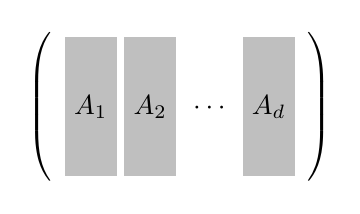
\begin{tikzpicture}
                        \matrix[hsupermatrix]{
                            \node[vsubmatrix] (a1) {A_1}; \& \node[vsubmatrix] (a2) {A_2}; \& \cdots \& \node[vsubmatrix] (ad) {A_d}; \\
                        };
                    \end{tikzpicture}
                \end{figure}
                \begin{figure}
                    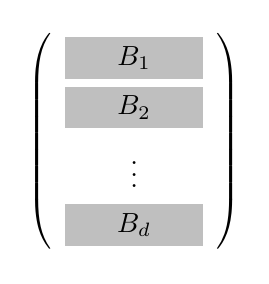
\begin{tikzpicture}
                        \matrix[vsupermatrix]{
                            \node[hsubmatrix] (b1) {B_1}; \\ \node[hsubmatrix] (b2) {B_2}; \\ \vdots \\ \node[hsubmatrix] (bd) {B_d}; \\
                        };
                    \end{tikzpicture}
                \end{figure}
            }
        \end{column}
    \end{columns}
\end{frame}

\begin{frame}{Theorem 3.2\footnote[1]{\cite{Chan2007}} \only<2>{\& Corollary 3.3\footnotemark[1]}}
    \begin{theorem}\label{thm:mat_mul}
        Given any two matrices $A, B \in \mathbb{R}^{n \times n}$ we can compute their min-plus (distance) product in a time of $\mathcal{O}\left( n^3 / \log(n) \right)$.
    \end{theorem}

    \uncover<2>{
        \begin{corollary}\label{cor:apsp_subcubic}
            We can solve the all pairs shortest paths problem for a graph with $\abs{V} = n$ nodes in $\mathcal{O}\left( n^3 / \log(n) \right)$ time.
        \end{corollary}
    }
\end{frame}
\section{Computing the Runtime}

\begin{frame}{Proof of Lemma~\ref{lem:dom_pairs}\footnote[1]{\cite[Lemma~2.1]{Chan2007}}}
    \setcounter{theorem}{0}
    \begin{lemma}
        Let $\mathbb{P} \subset \mathbb{R}^d$ be a set of red or blue points, partitioned into $\mathbb{P}_{red}$ and $\mathbb{P}_{blue}$ such that $n = \abs{\mathbb{P}_{red}} + \abs{\mathbb{P}_{blue}}$, and $\varepsilon \in \interval[open]{0}{1}$.
        Then we can find all $k$ dominating pairs in a time of $\mathcal{O}\left( c_\varepsilon^d n^{1 + \varepsilon} + k \right)$, where we define $c_\varepsilon := \frac{2^\varepsilon}{2^\varepsilon - 1}$.
    \end{lemma}
\end{frame}

\begin{frame}{Proof of Lemma~\ref{lem:dom_pairs}}
    \begin{exampleblock}{Assumption}
        All values are presorted by the $d$-th coordinate.
    \end{exampleblock}
\end{frame}

\begin{frame}{Proof of Lemma~\ref{lem:dom_pairs}}
    \emph{Idea: Divide and Conquer!}
    
    \uncover<1->{
        We split each set $\mathbb{P}_{red}$, $\mathbb{P}_{blue}$ along the median $d$-th coordinate into two sets each:
        \[
            \mathbb{P}_{red} \mapsto \mathbb{P}_{red, left}, \mathbb{P}_{red, right} \qquad \mathbb{P}_{blue} \mapsto \mathbb{P}_{blue, left}, \mathbb{P}_{blue, right}
        \]
    }
    \uncover<2->{
        such that it holds for all $p \in \mathbb{P}_{red}, q \in \mathbb{P}_{blue}$:
        \[
            p \in
            \begin{cases}
                \mathbb{P}_{red, left}, & p_d \leq m_d \\
                \mathbb{P}_{red, right}, & else
            \end{cases}
            \qquad
            q \in
            \begin{cases}
                \mathbb{P}_{blue, left}, & q_d \leq m_d \\
                \mathbb{P}_{blue, right}, & else
            \end{cases}
        \]

        Here, $m_d$ denote the median $d$-th coordinate for $\mathbb{P}_{red} \cup \mathbb{P}_{blue}$.
    }
\end{frame}

\begin{frame}{Proof of Lemma~\ref{lem:dom_pairs}}
    \emph{Idea: Divide and Conquer!}
    
    \begin{figure}
        \begin{tikzpicture}[scale=0.6, auto, swap]
            \only<1, 2, 3>{
                \foreach \pos / \name in {%
                    {(1, 1)/a}, {(4.5, 3.5)/b}%
                }%
                    \node[redpoint] (\name) at \pos {};
            }

            \only<1, 2, 4>{
                \foreach \pos / \name in {%
                    {(3, 0.5)/A}, {(2, 3)/B}, {(5, 5)/C}%
                }%
                    \node[bluepoint] (\name) at \pos {};
            }

            \only<3>{
                \foreach \pos / \name in {%
                    {(3, 0.5)/A}, {(2, 3)/B}, {(5, 5)/C}%
                }%
                    \node[bluepointalpha] (\name) at \pos {};

                \node[barlabel] (labelleft) at (-4, 5.5) {$\mathbb{P}_{red, left}$};
                \node[barlabel] (labelright) at (10, 5.5) {$\mathbb{P}_{red, right}$};
            }

            \only<4>{
                \foreach \pos / \name in {%
                    {(1, 1)/a}, {(4.5, 3.5)/b}%
                }%
                    \node[redpointalpha] (\name) at \pos {};

                \node[barlabel] (labelleft) at (-4, 5.5) {$\mathbb{P}_{blue, left}$};
                \node[barlabel] (labelright) at (10, 5.5) {$\mathbb{P}_{blue, right}$};
            }

            \only<2->{
                \node[ghost] (hook1) at (3, -.5) {};
                \node[ghost] (hook2) at (3, 6.5) {};

                \path[divides] (hook1) -- (hook2);
            }
            
            \only<3->{
                \node[ghost] (lefttarget) at (.5, 5.5) {};
                \node[ghost] (righttarget) at (5.5, 5.5) {};

                \path[points] (labelleft) -- (lefttarget);
                \path[points] (labelright) -- (righttarget);
            }

            \node[barlabel] (labelx) at (3, -0.75) {Coordinate 2};
            \node[barlabel, rotate=90] (labely) at (-0.75, 3) {Coordinate 1};

            \node[ghost] (bound1) at (0, 0) {};
            \node[ghost] (bound2) at (6, 6) {};

            % border
            \node[draw, fit=(bound1) (bound2)] (border) {};
        \end{tikzpicture}
    \end{figure}
\end{frame}

\begin{frame}{Proof of Lemma~\ref{lem:dom_pairs}}
    We solve the dominating pairs problem on the sets
    \[
        \mathbb{P}_{red, left} \cup \mathbb{P}_{blue, left}, \qquad \mathbb{P}_{red, right} \cup \mathbb{P}_{blue, right}, \qquad \mathbb{P}_{red, left} \cup \mathbb{P}_{blue, right}.
    \]
    (For the first $d - 1$ coordinates for the third set.)

    \uncover<2->{
        We do not consider $\mathbb{P}_{red, right} \cup \mathbb{P}_{blue, left}$, because $\forall p \in \mathbb{P}_{red, right}, q \in \mathbb{P}_{blue, left}: q_d \leq m_d \leq p_d$.
        Hence no $q$ can never dominate any $p$.
    }

    \uncover<3->{
        We stop dividing if the number of points left to consider is $1$; we output all pairs of red and blue points if the number of dimensions left is $0$.
    }
\end{frame}

\begin{frame}{Proof of Lemma~\ref{lem:dom_pairs}}
    \[
        \mathbb{P}_{red, left} \cup \mathbb{P}_{blue, left}, \qquad \mathbb{P}_{red, right} \cup \mathbb{P}_{blue, right}, \qquad \mathbb{P}_{red, left} \cup \mathbb{P}_{blue, right}
    \]

    We do not need to consider $\mathbb{P}_{red, right} \cup \mathbb{P}_{blue, left}$.

    \uncover<2->{
        \begin{figure}
            \centering
            \begin{tikzpicture}[scale=0.6, auto, swap]
                \only<2, 4>{\node[redpoint] (a) at (1, 1) {};}
                \only<3>{\node[redpoint] (b) at (4.5, 3.5) {};}

                \only<3, 4>{\node[bluepoint] (C) at (5, 5) {};}
                \only<2>{
                    \node[bluepoint] (A) at (3, 0.5) {};
                    \node[bluepoint] (B) at (2, 3) {};
                }

                \node[barlabel] (labelx) at (3, -0.75) {Coordinate 2};
                \node[barlabel, rotate=90] (labely) at (-0.75, 3) {Coordinate 1};

                \node[ghost] (bound1) at (0, 0) {};
                \node[ghost] (bound2) at (6, 6) {};

                \node[ghost] (hook1) at (3, -.5) {};
                \node[ghost] (hook2) at (3, 6.5) {};

                \path[divides] (hook1) -- (hook2);

                \node[ghost] (middlehook1) at (2.6, 6) {};
                \node[ghost] (middlehook2) at (3.4, 0) {};

                % alpha highlights
                \only<2, 4>{
                    \node[fill=red, fill opacity=.2, fit=(bound1) (middlehook1)] (redleft) {};
                    \only<2>{\node[fill=blue, fill opacity=.2, fit=(bound1) (middlehook1)] (blueleft) {};}
                }
                \only<3, 4>{
                    \node[fill=blue, fill opacity=.2, fit=(middlehook2) (bound2)] (blueright) {};
                    \only<3>{\node[fill=red, fill opacity=.2, fit=(middlehook2) (bound2)] (redright) {};}
                }

                % border
                \node[draw, fit=(bound1) (bound2)] (border) {};
            \end{tikzpicture}
        \end{figure}
    }
\end{frame}

\begin{frame}{Proof of Lemma~\ref{lem:dom_pairs}}
    Without the output costs of $\mathcal{O}\left( k \right)$, we get the recurrence relation
    \[
        T_d(n) \leq \underbrace{2 T_d\left( \frac{n}{2} \right)}_{(A)} + \underbrace{T_{d - 1}(n)}_{(B)} + \underbrace{\mathcal{O}(n)}_{(C)}.
    \]

    \uncover<2->{
        $(A)$: Two subproblems for half of the data each. $\leadsto \mathbb{P}_{red, left} \cup \mathbb{P}_{blue, left}, \mathbb{P}_{red, right} \cup \mathbb{P}_{blue, right}$

        $(B)$: Subproblem where d-th coordinate does not matter. $\leadsto \mathbb{P}_{red, left} \cup \mathbb{P}_{blue, right}$

        $(C)$: Time to split current point set about the median.\only<2->{\footnote[1]{\cite[Section~2.3.2]{Preparata1985}}}
    }

    \uncover<3>{
        From the termination criteria we get
        \[
            T_d(1) = \mathcal{O}\left( 1 \right), \qquad T_0(n) = \mathcal{O}\left( n \right).
        \]
    }

    % TODO: add images here to explain the degenerated case "all red points are left, all blue points are right"
\end{frame}

\begin{frame}{Proof of Lemma~\ref{lem:dom_pairs}}
    \[
        T_0(n) = \mathcal{O}\left( n \right)?
    \]

    ``If $d = 0$, we just output all pairs of red and blue points.''\only<1>{\footnote[1]{\cite[Lemma~2.1]{Chan2007}}}

    \uncover<2->{
        $\leadsto$ Output: $n^2$ pairs in the worst case \uncover<3->{$\implies T_0(n) = \mathcal{O}\left( n^2 \right)$}
    }

    \uncover<4->{
        $\leadsto$ Output: (\texttt{Pairs}, $\mathbb{P}_{red, left}$, $\mathbb{P}_{blue, right}$) in $\mathcal{O}(n)$\uncover<5->{, but postprocessing necessary later on!}
    }

    \uncover<6>{
        $\implies$ At some point we have to compute upto $\mathcal{O} \left( n^2 \right)$\dots
    }
\end{frame}

\begin{frame}{Proof of Lemma~\ref{lem:dom_pairs}}
    \[
        T_d(n) \leq 2 T_d\left( \frac{n}{2} \right) + T_{d - 1}(n) + \mathcal{O}(n)
    \]

    A first solution to this equation is that $T_d(n) = \mathcal{O}\left( n {\log(n)}^d \right)$, yielding an algorithmic runtime of $\mathcal{O}\left( n {\log(n)}^d + k \right)$. (Additional logarithmic factors can be safed by handling the cases $d = 1$ and $d = 2$ independently.\footnotemark[1]{})

    However, we can do better\dots
\end{frame}

\begin{frame}{Proof of Lemma~\ref{lem:dom_pairs}}
    \[
        T_d(n) \leq 2 T_d\left( \frac{n}{2} \right) + T_{d - 1}(n) + \mathcal{O}(n)
    \]

    Let $b$ be fixed, and define $T'(N) := \max \left\{ T_k(i) \,|\, i = 1, \dots, n; k = 1, \dots, d: b^k i \leq N \right\}$.
    
    Substituting into the previous reccurence formula thus yields for some constant $c$:
    \[
        T'(N) \leq 2 T'\left( \frac{N}{2} \right) + T'\left( \frac{N}{b} \right) + cN.
    \]
    
    \uncover<2>{
        $\implies$ What does this reccurence evaluate to and how do we need to choose $b$?
    }
\end{frame}

\begin{frame}{Proof of Lemma~\ref{lem:dom_pairs}}
    \[
        T'(N) \leq 2 T'\left( \frac{N}{2} \right) + T'\left( \frac{N}{b} \right) + cN
    \]

    \uncover<2->{
        By guessing that $T'(N) = \mathcal{O}\left( N^{1 + \varepsilon} - N \right) = \mathcal{O}\left( N^{1 + \varepsilon} \right)$, we get
        \begin{align*}
            T'(N) &\leq 2 \tilde{c} \left( {\left[ \frac{N}{2} \right]}^{1 + \varepsilon} - \frac{N}{2} \right) + \tilde{c} \left( {\left[ \frac{N}{b} \right]}^{1 + \varepsilon} - \frac{N}{b} \right) + cN \\
            \uncover<3->{
                &= \tilde{c} \left( \frac{2}{2^{1 + \varepsilon}} N^{1 + \varepsilon} - N \right) + \tilde{c} \left( \frac{1}{b^{1 + \varepsilon}} N^{1 + \varepsilon} - \frac{1}{b} N \right) + cN \\
            }
            \uncover<4->{
                &\leq \left( \frac{2}{2^{1 + \varepsilon}} + \frac{1}{b^{1 + \varepsilon}} \right) \tilde{c} N^{1 + \varepsilon} - \tilde{c} N - \frac{\tilde{c}}{b} N + cN.
            }
        \end{align*}
    }
\end{frame}

\begin{frame}{Proof of Lemma~\ref{lem:dom_pairs}}
    Thus far we computed
    \[
        T'(N) \leq \underbrace{\left( \frac{2}{2^{1 + \varepsilon}} + \frac{1}{b^{1 + \varepsilon}} \right)}_{(A)} \tilde{c} N^{1 + \varepsilon} - \tilde{c} N - \underbrace{\frac{\tilde{c}}{b} N + cN}_{(B)}.
    \]

    \uncover<2->{
        If $(A)$: $\begin{aligned}1 = \frac{2}{2^{1 + \varepsilon}} + \frac{1}{b^{1 + \varepsilon}}\end{aligned}$, and $(B)$: $c \leq \frac{\tilde{c}}{b}$ are fulfilled we get
        \[
            T'(N) \leq \tilde{c} N^{1 + \varepsilon} - \tilde{c} N \uncover<3->{\implies T'(N) = \mathcal{O}\left( N^{1 + \varepsilon} - N \right) = \mathcal{O}\left( N^{1 + \varepsilon} \right).}
        \]
    }

    \uncover<4>{
        It remains to calculate $b$.
    }
\end{frame}

\begin{frame}{Proof of Lemma~\ref{lem:dom_pairs}}
    If $(A)$: $\begin{aligned}1 = \frac{2}{2^{1 + \varepsilon}} + \frac{1}{b^{1 + \varepsilon}}\end{aligned}$, and $(B)$: $c \leq \frac{\tilde{c}}{b}$ are fulfilled we get
    \[
        T'(N) \leq \tilde{c} N^{1 + \varepsilon} - \tilde{c} N \implies T'(N) = \mathcal{O}\left( N^{1 + \varepsilon} - N \right) = \mathcal{O}\left( N^{1 + \varepsilon} \right).
    \]

    In $(A)$ we get $\begin{aligned}[t]
        1 = \frac{2}{2^{1 + \varepsilon}} + \frac{1}{b^{1 + \varepsilon}} &\iff b^{1 + \varepsilon} = b^{1 + \varepsilon} \frac{1}{2^\varepsilon} + 1 \iff -1 = \frac{b^{1 + \varepsilon}}{2^\varepsilon} - b^{1 + \varepsilon} \\
        &\iff -1 = \frac{1 - 2^\varepsilon}{2^\varepsilon} b^{1 + \varepsilon} \iff b^{1 + \varepsilon} = \frac{2^\varepsilon}{2^\varepsilon - 1} =: c_\varepsilon.
    \end{aligned}$
\end{frame}

\begin{frame}{Proof of Lemma~\ref{lem:dom_pairs}}
    We can now resubstitute:    
    \begin{align*}
        T'(N) &= \mathcal{O}\left( N^{1 + \varepsilon} - N \right) = \mathcal{O}\left( N^{1 + \varepsilon} \right) \\
        \implies T_d(n) &= \mathcal{O}\left( {\left( b^d n \right)}^{1 + \varepsilon} \right) = \mathcal{O}\left( c_\varepsilon^d n^{1 + \varepsilon} \right),
    \end{align*}
    because $T'(N) := \max \left\{ T_k(i) \,|\, i = 1, \dots, n; k = 1, \dots, d: b^k i \leq N \right\}$. 
    
    Finally, outputing all $k$ dominating pairs requires $\mathcal{O}\left( k \right)$ time. \qed{}
\end{frame}

\begin{frame}{Proof of Lemma~\ref{lem:sub_mat_mul}\footnote[1]{\cite[Lemma~3.1]{Chan2007}}}
    \setcounter{theorem}{1}
    \begin{lemma}
        Given two matrices $A \in \mathbb{R}^{n \times d}, B \in \mathbb{R}^{d \times n}$, and $\varepsilon \in \interval[open]{0}{1}, \begin{aligned}c_\varepsilon := \frac{2^\varepsilon}{2^\varepsilon - 1}\end{aligned}$, we can compute their min-plus product $A \otimes B$ in $\mathcal{O}\left( d c_\varepsilon^d n^{1 + \varepsilon} + n^2 \right)$ time.
    \end{lemma}
\end{frame}

\begin{frame}{Proof of Lemma~\ref{lem:sub_mat_mul}}
    \begin{exampleblock}{Note}
        We need to evaluate the inequality $a_{i, k} + b_{k, j} \leq a_{i, \tilde{k}} + b_{\tilde{k}, j}$.

        Ties such as $a_{i, k} + b_{k, j} = a_{i, \tilde{k}} + b_{\tilde{k}, j}$ are considered to be ``$<$'' if $k < \tilde{k}$.
    \end{exampleblock}
\end{frame}

\begin{frame}{Proof of Lemma~\ref{lem:sub_mat_mul}}
    \begin{exampleblock}{Reminder}
        We compute $C = A \otimes B$ elementwise through $c_{i, j} = \min\limits_k a_{i, k} + b_{k, j}$.
    \end{exampleblock}

    \uncover<2->{
        Consider $A$ to have entries ${\left( a_{i, j} \right)}_{i, j = 1}^{n, d}$, and $B$ to have entries ${\left( b_{i, j} \right)}_{i, j = 1}^{d, n}$.
        We want to compute the pairs
        \[
            X_k = \{ (i, j) \,|\, \forall k' = 1, \dots, d: a_{i, k} + b_{k, j} \leq a_{i, k'} + b_{k', j} \}
        \]
    }

    \uncover<3->{
        After computing these $X_k$, we can then set $C = A \otimes B$ elementwise as follows:

        For $(i, j) \in X_K$ we set $c_{i, j} = a_{i, k} + b_{k, j}$.
    }
\end{frame}

\begin{frame}{Proof of Lemma~\ref{lem:sub_mat_mul}}
    \begin{align*}
        X_k &= \{ (i, j) \,|\, \forall k' = 1, \dots, d: a_{i, k} + b_{k, j} \leq a_{i, k'} + b_{k', j} \} \\
            \uncover<2->{&= \{ (i, j) \,|\, \forall k' = 1, \dots, d: a_{i, k} - a_{i, k'} \leq b_{k', j} - b_{k, j} \}}
    \end{align*}
    \uncover<3->{
        This effectively amounts to computing all dominant pairs between the sets
        \begin{align*}
            \mathcal{A}_k &:= {\left\{ (a_{i, k} - a_{i, 1}), (a_{i, k} - a_{i, 2}), \dots, (a_{i, k} - a_{i, d}) \right\}}_{i = 1}^{n}, \text{and} \\
            \mathcal{B}_k &:= {\left\{ (b_{1, j} - b_{k, j}), (b_{2, j} - b_{k, j}), \dots, (b_{d, j} - b_{k, j}) \right\}}_{j = 1}^{n},
        \end{align*}
        where $\mathcal{A}_k$ takes the role of red points and $\mathcal{B}_k$ acts as the set of blue points.
    }

    \uncover<4>{
        By Lemma~\ref{lem:dom_pairs}, this takes an effort of $\mathcal{O}\left( c_\varepsilon^d n^{1 + \varepsilon} + \abs{X_k} \right)$.
    }
\end{frame}

\begin{frame}{Proof of Lemma~\ref{lem:sub_mat_mul}}
    \begin{exampleblock}{Note}
        It is possible to recover the shortest paths from the construction of the $X_k$s.
        We will see more on this later.
    \end{exampleblock}

    \uncover<2->{
        The penultimate step is to compute that
        \begin{align*}
            \mathcal{O}\left( \sum\limits_{k = 1}^d \left( c_\varepsilon^d n^{1 + \varepsilon} + \abs{X_k} \right) \right) = \mathcal{O}\left( d c_\varepsilon^d n^{1 + \varepsilon} + \sum\limits_{k = 1}^d \abs{X_k} \right),
        \end{align*}
        leaving only to compute that $\begin{aligned}\sum\limits_{k = 1}^d \abs{X_k}\end{aligned} = n^2$.
    }
\end{frame}

\begin{frame}{Proof of Lemma~\ref{lem:sub_mat_mul}}
    Suppose an index pair $(i, j)$ were to be included in $X_k$, and in $X_{\tilde{k}}$, with $k \neq \tilde{k}$.

    \uncover<2->{
        Recall the definition of $X_k$: 
        \[
            X_k = \{ (i, j) \,|\, \forall k' = 1, \dots, d: a_{i, k} + b_{k, j} \leq a_{i, k'} + b_{k', j} \}.
        \]

        Thus we get that $a_{i, k} + b_{k, j} \leq a_{i, \tilde{k}} + b_{\tilde{k}, j}$, because $(i, j) \in X_k$.
    }

    \uncover<3->{
        Applying the definition of $X_{\tilde{k}}$, we then also get $a_{i, \tilde{k}} + b_{\tilde{k}, j} \leq a_{i, k} + b_{k, j}$.
    }

    \uncover<4->{
        This means that $a_{i, \tilde{k}} + b_{\tilde{k}, j} = a_{i, k} + b_{k, j}$.

        To break this tie, we can w.l.o.g.\ assume $k < \tilde{k}$, which would result in $(i, j) \not\in X_{\tilde{k}}$.
    }

    \uncover<5>{
        $\implies$ Every index pair $(i, j)$ can only be included in at most one $X_k$.
    }
\end{frame}

\begin{frame}{Proof of Lemma~\ref{lem:sub_mat_mul}}
    Now assume that there would exist an index pair $(i, j)$ that is contained in none of the $X_k$.
    (Recall $X_k = \{ (i, j) \,|\, \forall k' = 1, \dots, d: a_{i, k} + b_{k, j} \leq a_{i, k'} + b_{k', j} \}$.)
    
    \uncover<2->{
        This is equivalent to the condition that
        \[
            \forall k = 1, \dots, d: \exists k' = 1, \dots, d: a_{i, k} + b_{k, j} > a_{i, k'} + b_{k', j}.
        \]
    }

    \uncover<3->{
        Because of the finite set we can choose $\hat{k} := \argmin\limits_{l = 1, \dots, d} a_{i, l} + b_{l, j}$.
    }

    \uncover<4->{
        Hence, choosing $k = \hat{k}$ yields $\forall k' = 1, \dots, d: a_{i, k} + b_{k, j} = a_{i, \hat{k}} + b_{\hat{k}, j} \leq a_{i, k'} + b_{k', j}$. \Lightning{}
    }
    
    \uncover<5>{
        $\implies$ Every index pair $(i, j)$ has to be included in one $X_k$.
    }
\end{frame}

\begin{frame}{Proof of Lemma~\ref{lem:sub_mat_mul}}
    \begin{alertblock}{Recall}
        Every index pair $(i, j)$ can only be included in at most one $X_k$.

        Every index pair $(i, j)$ has to be included in one $X_k$.
    \end{alertblock}
    
    $\implies$ Over all $X_k, k = 1, \dots, d$, every index pair $(i, j)$ is encountered exactly once.

    \uncover<2>{
        $\implies \begin{aligned}\sum\limits_{k = 1}^d \abs{X_k}\end{aligned} = n^2$

        $ \implies \mathcal{O}\left( \sum\limits_{k = 1}^d \left( c_\varepsilon^d n^{1 + \varepsilon} + \abs{X_k} \right) \right) = \mathcal{O}\left( d c_\varepsilon^d n^{1 + \varepsilon} + n^2 \right)$ \qed{}
    }
\end{frame}

\begin{frame}{Proof of Theorem~\ref{thm:mat_mul}\footnote[1]{\cite[Theorem~3.2]{Chan2007}}}
    \setcounter{theorem}{2}
    \begin{theorem}
        Given any two matrices $A, B \in \mathbb{R}^{n \times n}$ we can compute their min-plus (distance) product in a time of $\mathcal{O}\left( n^3 / \log(n) \right)$.
    \end{theorem}
\end{frame}

\begin{frame}{Proof of Theorem~\ref{thm:mat_mul}}
    We recall the idea of splitting matrices to multiply them:

    \begin{columns}
        \begin{column}{.2\linewidth}
            \begin{figure}
                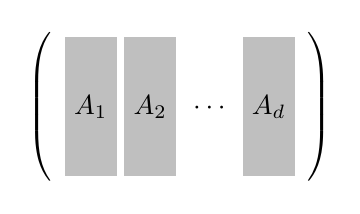
\begin{tikzpicture}
                    \matrix[hsupermatrix]{
                        \node[vsubmatrix] (a1) {A_1}; \& \node[vsubmatrix] (a2) {A_2}; \& \cdots \& \node[vsubmatrix] (ad) {A_d}; \\
                    };
                \end{tikzpicture}
            \end{figure}
        \end{column}
        \begin{column}{.2\linewidth}
            \begin{figure}
                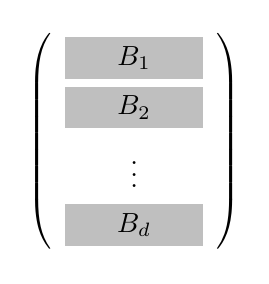
\begin{tikzpicture}
                    \matrix[vsupermatrix]{
                        \node[hsubmatrix] (b1) {B_1}; \\ \node[hsubmatrix] (b2) {B_2}; \\ \vdots \\ \node[hsubmatrix] (bd) {B_d}; \\
                    };
                \end{tikzpicture}
            \end{figure}
        \end{column}
    \end{columns}

    $\implies$ Strassen is not applicable here --- we need to make use of the relation between matrix multiplication and matrix closure.
\end{frame}

\begin{frame}{Proof of Theorem~\ref{thm:mat_mul}}
    We split our matrices $A$ and $B$ into $\begin{aligned}\frac{n}{d}\end{aligned}$ blocks, that is $\begin{aligned}\forall l = 1, \dots, \frac{n}{d}: A_l \in \mathbb{R}^{n \times d}, B_l \in \mathbb{R}^{d \times n}\end{aligned}$ for some fixed $d$.
    (If necessary we round $\begin{aligned}\frac{n}{d}\end{aligned}$ and adjust the number of blocks accordingly.)

    \uncover<2->{
        We then compute the distance products $A_i \otimes B_i$ for all $\begin{aligned}i = 1, \dots, \frac{n}{d}\end{aligned}$, and set the product to be defined by the element-wise minimum, i.e.\ $\begin{aligned}[t]c_{i, j} := \min\limits_{l = 1, \dots, \frac{n}{d}} {\left( A_l \otimes B_l \right)}_{i, j}\end{aligned}$, where $i, j = 1, \dots, n$.
    }

    \uncover<3->{
        By Lemma~\ref{lem:sub_mat_mul}, this procedure requires $\begin{aligned}\mathcal{O}\left( \frac{n}{d} \left( d c_\varepsilon^d n^{1 + \varepsilon} + n^2 \right) \right) = \mathcal{O} \left( c_\varepsilon^d n^{2 + \varepsilon} + \frac{n^3}{d} \right)\end{aligned}$ time.
    }

    \uncover<4->{
        It now only remains to choose the constant $d$.
    }
\end{frame}

\begin{frame}{Proof of Theorem~\ref{thm:mat_mul}}
    We want to assure $\begin{aligned}\frac{n^3}{d} > c_\varepsilon^d n^{2 + \varepsilon}\end{aligned}$.

    \uncover<2->{
        The choice of $d = \tilde{c} \log(n)$ for $\tilde{c}$ sufficiently small and depending on $\varepsilon$ is useful because
        \begin{itemize}
            \item $C^{D \log(n)} \sim n^D$ grows polynomially, whereas e.\ g.
            \item<3-> $C^n$ grows exponentially.
        \end{itemize}
    }

    \uncover<4->{
        We then get
        $\begin{aligned}
            \mathcal{O}\left( c_\varepsilon^d n^{2 + \varepsilon} + \frac{n^3}{d} \right) = \mathcal{O}\left( \frac{n^3}{\log(n)} \right)
        \end{aligned}$. \qed{}
    }

    \uncover<5>{
        One possible choice is $\varepsilon \approx 0.38, c_\varepsilon \approx 4.32, d \approx 0.42 \log(n)$\footnotemark[1].
    }
\end{frame}

\begin{frame}{Proof of Corollary~\ref{cor:apsp_subcubic}\footnote[1]{\cite[Corollary~3.3]{Chan2007}}}
    \setcounter{theorem}{3}
    \begin{corollary}
        We can solve the all pairs shortest paths problem for a graph $G = (V, E)$ with $\abs{V} = n$ nodes in $\mathcal{O}\left( n^3 / \log(n) \right)$ time.
    \end{corollary}
\end{frame}

\begin{frame}{Proof of Theorem~\ref{cor:apsp_subcubic}}
    We consider $A$ and $B$ to be the matrices defined by $\begin{aligned}d(i, j) := \begin{cases}
        w(e), &\exists e \in E: e = (i, j) \\
        \infty, &else
    \end{cases}\end{aligned}$.

    The corollary then follows by applying Theorem~\ref{thm:mat_mul}. \qed{}
\end{frame}
\section{Recovery of Shortest Paths and Setting Product Matrix Entries}

\begin{frame}{Recovery of Shortest Paths}
    We want to recover a shortest path from vertex $i$ to vertex $j$.
    Consider $(i, j) \in X_k$.

    \uncover<2->{
        This means that a shortest path from $i$ to $j$ must go through $k$ because $\forall k' = 1, \dots, n: w_{i, k} + w_{k, j} \leq w_{i, k'} + w_{k', j}$.

        (\emph{Taking a path through any vertex other than $k$ increases the weight.})
    }

    \uncover<3->{
        For neighbouring vertices, where a shortest path is the edge directly between them, we get that $(i, j) \in X_m$, with $m = \min \{ i, j \}$ because (assuming $i < j$) $\forall k' = 1, \dots, n: w_{i, i} + w_{i, j} \leq w_{i, k'} + w_{k', j}$.

        (\emph{Direct shortest paths between neighbouring vertices $i$ and $j$ fall into $X_i$ or $X_j$.})
    }
\end{frame}

\begin{frame}{Recovery of Shortest Paths}
    \begin{algorithm}[H]
        \KwData{The sets $X_k$, source vertex $i$, target vertex $j$}
        \SetKwProg{myproc}{def}{}{}
        \myproc{get\_shortest\_path$(i, j)$}{
            Set $k$ such that $(i, j) \in X_k$\;
            \If{$k \not\in \{ i, j \}$}{
                Set $\mathfrak{p} := $ \emph{get\_shortest\_path}$(i, k)$ $\oplus$ \emph{get\_shortest\_path}$(k, j)$\;
            }
            \Else{
                Set $\mathfrak{p} := (i, j)$\;
            }
            \Return{$\mathfrak{p}$}
        }
    \end{algorithm}

    With the usual definition $(a, \dots, b) \oplus (b, \dots, c) := (a, \dots, b, \dots, c)$.
\end{frame}

\begin{frame}{Setting the Product Matrix' Entries $c_{i, j}$\only<1>{\footnote[1]{\cite{Chan2007}}}}
    Setting $c_{i, j} = a_{i, k} + b_{k, j}$ directly is not going to work due to random access constraints.\only<1>{\footnotemark[1]}

    \uncover<2->{
        Instead we consider a ``bucket'' $\mathcal{B}_i$ for every $i = 1, \dots, n$ and an additional ``slot'' matrix $S$ of dimension $n \times n$.
    }

    \uncover<3->{
        For $(i, j) \in X_k$ we insert $(j, k)$ into $\mathcal{B}_i$ in $\mathcal{O}\left( n^2 \right)$ time.
    }

    \uncover<4->{
        For every $i = 1, \dots, n$ we presort the bucket $\mathcal{B}_i$ with respect to the first index in $\mathcal{O}\left( n \log(n) \right)$ time.
        (\emph{This corresponds to the $j$ from the index pairs above.})
    }

    \uncover<5->{
        We then set the entry $s_{i, j}$ to $k$ for every $(j, k) \in \mathcal{B}_i$ in $\mathcal{O}\left( n^2 \right)$ time.
    }

    \uncover<6->{
        Finally, we can set $c_{i, j} = a_{i, s_{i, j}} + b_{s_{i, j}, j}$ in $\mathcal{O}\left( n^2 \right)$ time.

        In total, this results in $\mathcal{O}\left( 3 n^2 + n \log(n) \right) = \mathcal{O}\left( n^2 \right)$.
    }
\end{frame}


\section*{Summary \& Discussion}

\begin{frame}{Summary \& Discussion}
    \begin{enumerate}
        \item Computing dominating pairs $\mathcal{O}\left( c_\varepsilon^d n^{1 + \varepsilon} + k \right)$
        \item Computing $A \otimes B$ for rectangular matrices $\mathcal{O}\left( d c_\varepsilon^d n^{1 + \varepsilon} + n^2 \right)$
        \item Computing $A \otimes B$ for quadratic matrices $\begin{aligned}[t]\mathcal{O}\left( \frac{n^3}{\log(n)} \right)\end{aligned}$
        \item Making the jump to APSP problems
    \end{enumerate}

    \begin{algorithm}[H]
        \KwData{Weight matrix $W$}
        Split $W$ into $W_1, \dots, W_{\frac{n}{d}}$\;
        \For{$i = 1, \dots, \frac{n}{d}$}{
            Compute the min-plus products $W_i \otimes W_i$\;
            \Indp{}
            Create the index sets $X_k$\;
            Recover the product matrix' entries via bins/buckets\;
            \Indm{}
        }
        Set the final shortest paths matrix elementwise as the minimum over the $W_i \otimes W_i$\;
    \end{algorithm}
\end{frame}

\end{document}
